\section{Introduction}

\subsection{What is Etherbone?}

Etherbone is an open source project developed by GSI \cite{gsi} that allows low level access features to the different Wishbone peripheral existing in FPGA design. GSI has developed gateware and software for this task. The Etherbone core is an IP core that must be added in your design if you want to access your device from the network. On the other hand, GSI has developed a software library that uses Linux/Unix network sockets (it is based on UDP/TCP packets) to communicate with the Etherbone core and write/read from the device memory map. 
Finally, if you want to use Etherbone to configure your device, you must add the Etherbone core into your gateware and use the Etherbone library to send/receive packets to/from network. You can get more information in \cite{Etherbone-repo}. 

\subsection{What is CALoE?}

CALoE, Configuration Abstraction Layer over Etherbone, is a library based on Etherbone that permits remote control of SPEC cards \cite{Spec-board} and other devices with Etherbone core.
However, high level commands are not supported by Etherbone. UGR has designed and implemented a higher level library over Etherbone (CALoE) to ease work to programmer/developer. CALoE libray can be used to define an input configuration file in which you can specify a set of operations 
of your card/device and then, CALoE reads it and you can call your operations as C functions. 

Figure \ref{caloe_layer_model_img} describes layer model of CALoE library. User applications are implemented by using CALoE API and must include any device user configuration files.

\begin{figure}[H]
\centering
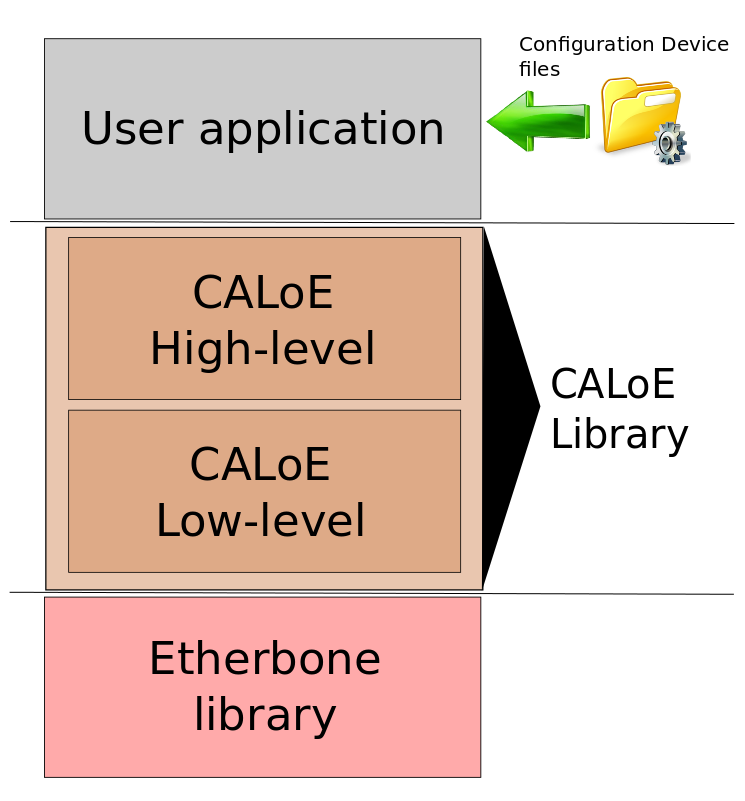
\includegraphics[width=150px,height=200px]{img/layer_model.png}
\caption{CALoE layer model}
\label{caloe_layer_model_img}
\end{figure}

CALoE has been developed by University of Granada (UGR) and is written in C/C++. It is published under LGPLv3 license. All source files are available in OHWR repository in the starting kit project, ugr branch (see in \cite{WR-starting-kit}).

In the next sections, we describe features of CALoE library.
